\chapter{Proposed Solution}
\section{Introduction}
This chapter is devoted to present our proposed solution to index data and make an \textbf{EDA} as well as 
implementing the solution in a distributed way.

\section{Architecture of the solution}
\subsection{Distributed Architecture}
\subsubsection{Definition}
A distributed system is a system whose components are located on different networked computers, which communicate and coordinate their actions by passing messages to one another.\\ 
The components interact with one another in order to achieve a common goal.
 
\subsubsection{Benefits}
Using a distributed architecture can make our life much easier, because it provides: \\
\begin{itemize}
    \item \textbf{Scaling}: Distributed Systems are easily scalable.
    \item \textbf{Prallelism}: Distributed Systems are designed for parallelism.
    \item \textbf{Reliability}: Distributed Systems can tolerate hardware failures.
\end{itemize}
\cleardoublepage
\subsection{Logical architecture}
In this section we present, the logical architecture of our framework to index investment data provided by MAJESTEYE.
\begin{itemize}
    \item \textbf{Zookeeper Ensemble}: 3 Zookeeper instances to synchronize \textit{Solr} nodes.
    \item \textbf{Apache Solr}: 5 Solr nodes used to index data.
    \item \textbf{Hadoop (HDFS)}: 1 NameNode and 2 DataNode used to store index and provide easy scaling.
\end{itemize}

\subsection{Docker (Physical Architecture)}
all instances are running under \textbf{Docker Engine} to simulate a Mini-Cloud Environnement.
\subsubsection{Definition}
Docker is a set of platform as a service (PaaS) products that uses OS-level virtualization to deliver software in packages called containers.
\subsubsection{Docker Conatiner}
A container is a standard unit of software that packages up code and all its dependencies so the application runs quickly and reliably from one computing environment to another. \\A Docker container image is a lightweight, standalone, executable package of software that includes everything needed to run an application: code, runtime, system tools, system libraries and settings.
\begin{center}
    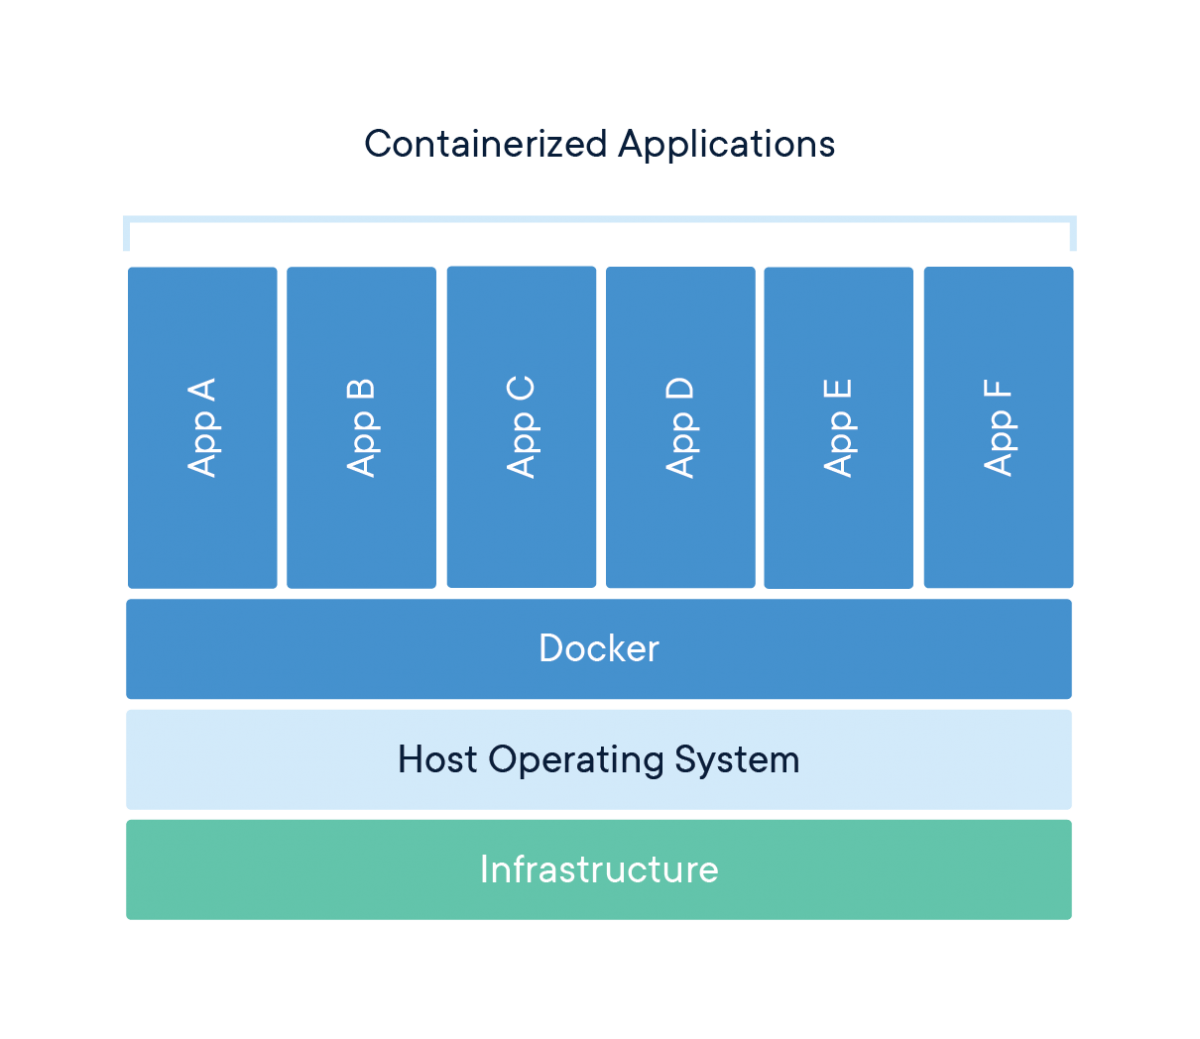
\includegraphics[scale=0.2]{images/container.png}
\end{center}
\subsubsection{Benefits}
Docker Containers are:
\begin{itemize}
    \item \textbf{Standard}: Docker created the industry standard for containers, so they could be portable anywhere.
    \item \textbf{Lightweight}: Containers share the machine’s OS system kernel and therefore do not require an OS per application.
    \item \textbf{Secure}:  Applications are safer in containers and Docker provides the strongest default isolation capabilities in the industry.
\end{itemize}

\clearpage

\section{Software Environnement}
\subsection{Apache Zookeeper}
\begin{wrapfigure}[8]{r}{4cm}
    
\includegraphics[width=4cm]{images/zookeeper.jpeg}
    \end{wrapfigure}
ZooKeeper is a centralized service for maintaining configuration information, naming, providing distributed synchronization, and providing group services. \\
All of these kinds of services are used in some form or another by distributed applications. Each time they are implemented there is a lot of work that goes into fixing the bugs and race conditions that are inevitable.\\
Because of the difficulty of implementing these kinds of services, applications initially usually skimp on them, which make them brittle in the presence of change and difficult to manage. Even when done correctly, different implementations of these services lead to management complexity when the applications are deployed.
\bigbreak
\bigbreak
\bigbreak
\bigbreak
\bigbreak
\bigbreak
\subsection{Apache Solr}
As mentioned below we will be using Apache Solr for indexing our investment dataset.
\subsection{Apache Hadoop}

